% Capítulo 10: busca binária por 41 em um vetor ordenado de 15 elementos.
\documentclass[border=4pt]{standalone}
\usepackage[utf8]{inputenc}
\usepackage[T1]{fontenc}
% Estilo comum das figuras de vetores (capítulo 8).
\usepackage{tikz}
\usetikzlibrary{arrows.meta, positioning, calc, decorations.pathreplacing}
\definecolor{navy}{RGB}{23,45,80}
\definecolor{laranja}{RGB}{250,110,29}
\definecolor{cinzalogo}{RGB}{107,114,126}
\definecolor{azul}{RGB}{205,222,247}
\tikzset{
  casa/.style={draw=navy, line width=0.9pt, minimum width=8mm, minimum height=7mm,
               inner sep=0pt, font=\sffamily\small},
  pronta/.style={casa, fill=azul},
  parte/.style={casa, fill=laranja!12},
  marcada/.style={casa, fill=laranja!45, draw=laranja},
  fora/.style={casa, draw=cinzalogo!60, dashed, fill=white, text=cinzalogo!60},
  indice/.style={font=\sffamily\scriptsize, text=cinzalogo},
  explica/.style={font=\sffamily\small, text=navy, anchor=east},
  legenda/.style={font=\sffamily\scriptsize, text=cinzalogo},
  rotulo/.style={font=\sffamily\small\bfseries, text=navy},
  seta/.style={-{Stealth[length=2.2mm]}, navy, line width=0.9pt},
  chave/.style={decorate, decoration={brace, amplitude=4pt, mirror}, navy, line width=0.8pt},
}
% \vetor{nome}{x}{y}{valor/estilo, valor/estilo, ...}: casas lado a lado, chamadas nome0, nome1...
\newcommand{\vetor}[4]{%
  \foreach \valor/\estilo [count=\i from 0] in {#4} {
    \node[\estilo] (#1\i) at ($(#2, #3) + (\i*0.8, 0)$) {\valor};
  }
}

\tikzset{passo/.style={font=\sffamily\scriptsize, text=navy, anchor=west, align=left}}
\begin{document}
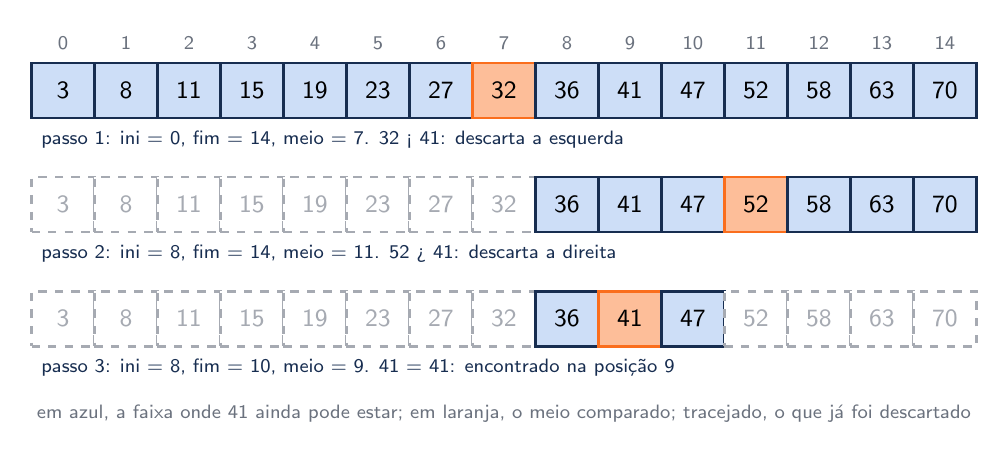
\begin{tikzpicture}
  \node[indice] at (0.0, 0.6) {0};
  \node[indice] at (0.8, 0.6) {1};
  \node[indice] at (1.6, 0.6) {2};
  \node[indice] at (2.4000000000000004, 0.6) {3};
  \node[indice] at (3.2, 0.6) {4};
  \node[indice] at (4.0, 0.6) {5};
  \node[indice] at (4.800000000000001, 0.6) {6};
  \node[indice] at (5.6000000000000005, 0.6) {7};
  \node[indice] at (6.4, 0.6) {8};
  \node[indice] at (7.2, 0.6) {9};
  \node[indice] at (8.0, 0.6) {10};
  \node[indice] at (8.8, 0.6) {11};
  \node[indice] at (9.600000000000001, 0.6) {12};
  \node[indice] at (10.4, 0.6) {13};
  \node[indice] at (11.200000000000001, 0.6) {14};
  \vetor{p0}{0}{0.0}{3/pronta, 8/pronta, 11/pronta, 15/pronta, 19/pronta, 23/pronta, 27/pronta, 32/marcada, 36/pronta, 41/pronta, 47/pronta, 52/pronta, 58/pronta, 63/pronta, 70/pronta}
  \node[passo] at (-0.4, -0.62) {passo 1: ini = 0, fim = 14, meio = 7. 32 < 41: descarta a esquerda};
  \vetor{p1}{0}{-1.45}{3/fora, 8/fora, 11/fora, 15/fora, 19/fora, 23/fora, 27/fora, 32/fora, 36/pronta, 41/pronta, 47/pronta, 52/marcada, 58/pronta, 63/pronta, 70/pronta}
  \node[passo] at (-0.4, -2.07) {passo 2: ini = 8, fim = 14, meio = 11. 52 > 41: descarta a direita};
  \vetor{p2}{0}{-2.9}{3/fora, 8/fora, 11/fora, 15/fora, 19/fora, 23/fora, 27/fora, 32/fora, 36/pronta, 41/marcada, 47/pronta, 52/fora, 58/fora, 63/fora, 70/fora}
  \node[passo] at (-0.4, -3.52) {passo 3: ini = 8, fim = 10, meio = 9. 41 = 41: encontrado na posição 9};
  \node[legenda] at (5.6, -4.1) {em azul, a faixa onde 41 ainda pode estar; em laranja, o meio comparado; tracejado, o que já foi descartado};
\end{tikzpicture}
\end{document}
